\documentclass[12pt]{article}

\usepackage[margin=1in]{geometry}
\usepackage{graphicx}
\usepackage{booktabs}
\usepackage{amsmath}

\title{The Effect of Paid Search Advertising on Revenue: \\
A Replication of the eBay Natural Experiment}
\author{Ese Okitiakpe}
\date{March 5, 2026}

\begin{document}

\maketitle

\section{Introduction}

Paid search advertising is widely used by firms to attract consumers through search engines such as Google. Companies spend billions of dollars on search engine marketing (SEM), but it is often difficult to know whether these ads actually increase revenue or whether they simply capture users who would have visited the website anyway. The research question in this paper is whether paid search advertising has a meaningful effect on eBay’s revenue. Blake, Nosko, and Tadelis (2014) study this question using a natural experiment in which eBay temporarily stopped bidding on paid search advertisements in some markets. In this replication, a difference-in-differences (DID) approach to estimate the causal effect of paid search advertising on revenue.

\section{Experimental Setting}

Blake et al. (2014) worked with eBay to run a large-scale field experiment to measure the impact of paid search advertising. In the experiment, eBay stopped bidding on Google AdWords advertisements in a subset of U.S. designated market areas (DMAs). Specifically, 65 out of 210 DMAs were selected for treatment starting on May 22, 2012. In those treatment markets, paid search advertising was turned off, meaning that search\_stays\_on equals zero. The remaining DMAs continued running paid search advertisements and served as the control group, where search\_stays\_on equals one. The treatment lasted for about eight weeks.

It is important to note that this was not a fully randomized experiment. The largest DMAs were excluded from the treatment group because they represent a large share of eBay’s total revenue. Because of this, the treatment and control groups differ in their baseline revenue levels. A simple comparison of average revenue between the two groups would therefore be misleading. Instead, the analysis uses a difference-in-differences approach, which compares how revenue changes over time in the treatment markets relative to the control markets.

\section{Data and Figures}

The dataset contains daily revenue observations for 210 DMAs from April to July 2012. Each observation includes the date, the DMA identifier, whether the market belongs to the treatment or control group, and the revenue generated in that market. The treatment period began on May 22, 2012, when paid search advertising was turned off in the treatment markets. These data allow us to compare revenue trends before and after the intervention across both treatment and control groups.

\begin{figure}[h]
    \centering
    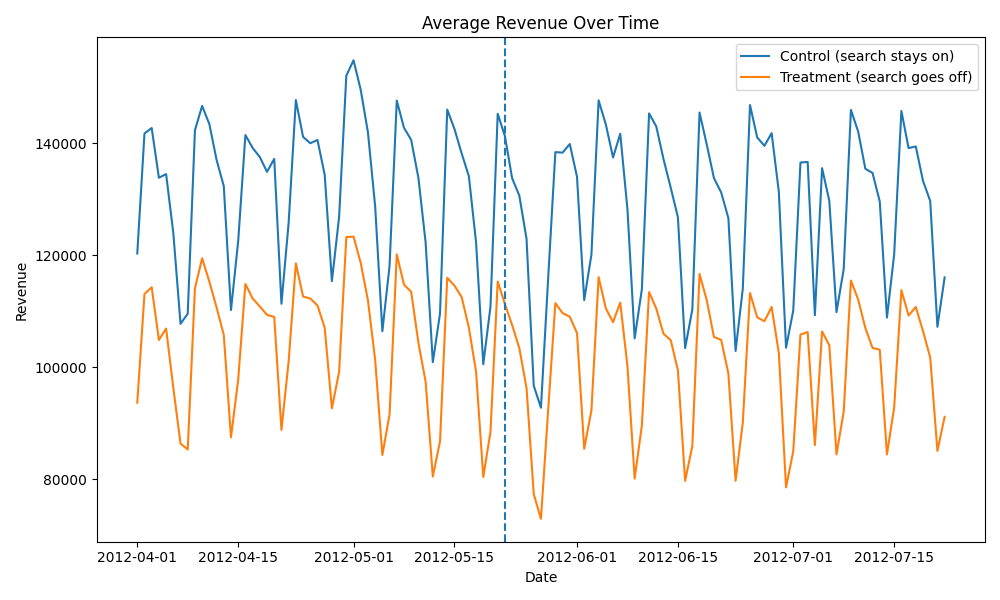
\includegraphics[width=0.85\textwidth]{../output/figures/figure_5_2.png}
    \caption{Average revenue for treatment and control DMAs over time.
             The dashed line marks May 22, 2012, when SEM was turned off
             for the treatment group.}
    \label{fig:revenue}
\end{figure}


Figure \ref{fig:revenue} shows the average revenue for treatment and control DMAs over time. The control group consistently has higher revenue levels because the largest DMAs were excluded from the treatment group. Despite this difference in levels, both groups show similar weekly patterns in revenue, which suggests that consumer activity follows similar cycles across markets. At this scale, it is difficult to clearly see a divergence between the treatment and control groups after May 22.


\begin{figure}[h]
    \centering
    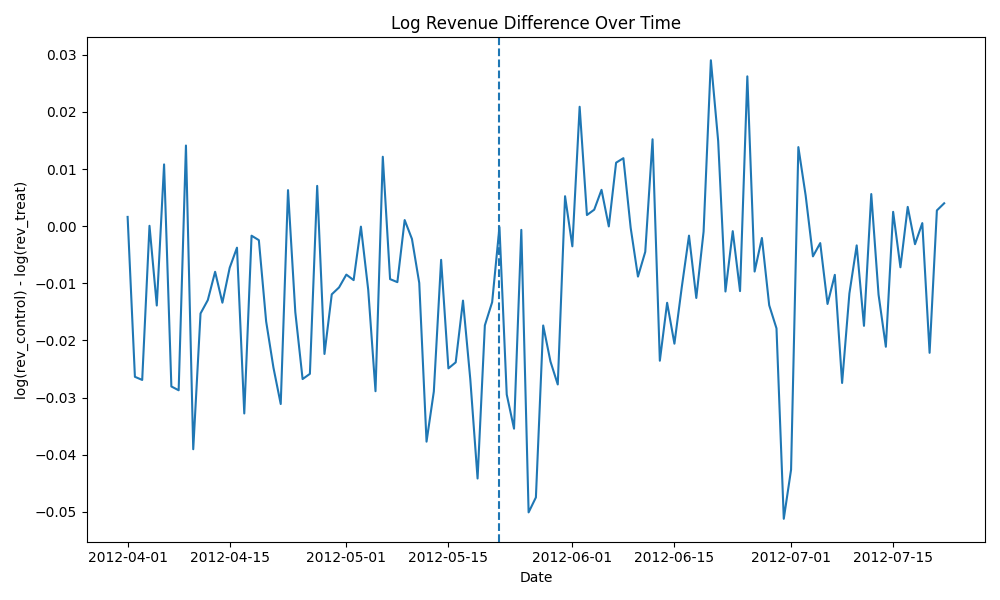
\includegraphics[width=0.85\textwidth]{../output/figures/figure_5_3.png}
    \caption{Log-scale average revenue difference between control and treatment
             groups over time. The gap appears to increase after May 22.}
    \label{fig:logdiff}
\end{figure}


Figure \ref{fig:logdiff} plots the log difference between average control and treatment revenue over time. Before May 22, the difference fluctuates around a relatively stable level. After the treatment date, the gap appears to increase slightly, suggesting that revenue in treatment markets may have declined relative to the control markets once paid search advertising was turned off. While the change is small, this pattern motivates estimating the treatment effect more formally using a DID framework.


\section{Results}



\input{../output/tables/did_table.tex}


Table \ref{tab:did} reports the difference-in-differences estimate of the effect of paid search advertising on revenue. The estimated treatment effect in log scale is approximately $\hat{\gamma} = -0.0066$. Converting this estimate to levels gives $exp(-0.0066) \approx 0.9934$, which implies that turning off paid search advertising reduced revenue in the treatment markets by about 0.66 percent.

However, the 95\% confidence interval ranges from $-0.0175$ to $0.0043$, which includes zero. This means the estimate is not statistically significant at the 5 percent level. In economic terms, the results suggest that paid search advertising has only a very small effect on eBay’s revenue. One possible explanation is that many users who click on paid search ads would have found eBay through organic search results even without the advertisements.

\section{Conclusion}

Overall, the difference-in-differences analysis finds a small and statistically insignificant effect of paid search advertising on revenue. This result is consistent with the main finding of Blake et al. (2014), which suggests that paid search advertising may have limited incremental value for a well-known brand like eBay. One limitation of this replication is that the revenue data used in the analysis are scaled rather than representing actual revenue values. In addition, the treatment was not fully randomized, and the analysis relies on a simple DID approach rather than a regression with additional controls. Even so, the results highlight how difficult it can be to measure the true return on investment from advertising.


\begin{thebibliography}{9}
\bibitem{blake2014}
Blake, T., C. Nosko, and S. Tadelis (2014).
``Consumer Heterogeneity and Paid Search Effectiveness: A Large-Scale Field Experiment.''
\textit{Econometrica}, 83(1): 155--174.

\bibitem{taddy2019}
Taddy, M. (2019).

\textit{Business Data Science}. McGraw-Hill, Chapter 5.
\end{thebibliography}

\end{document}


